\documentclass[11pt]{article}
\usepackage[T1]{fontenc}
\usepackage[utf8]{inputenc}
\usepackage{lmodern}
\usepackage[margin=1in]{geometry}
\usepackage{amsmath,amssymb,amsthm,mathtools}
\usepackage{booktabs,longtable,array}
\usepackage{graphicx}
\usepackage{xcolor}
\usepackage{microtype}
\usepackage{enumitem}
\usepackage{listings}
\usepackage{hyperref}
\usepackage{fancyhdr}
\definecolor{ink}{HTML}{17344A}
\definecolor{linkblue}{HTML}{1C627F}
\hypersetup{colorlinks=true,linkcolor=linkblue,citecolor=linkblue,urlcolor=linkblue,
 pdftitle={A quantitative constructive implicit function theorem in iPRA},
 pdfauthor={Research note prepared for Vladimir Reshetnikov}}
\pagestyle{fancy}\fancyhf{}
\fancyhead[L]{\small\color{ink}Constructive implicit functions in iPRA}
\fancyhead[R]{\small November 21, 2026}
\fancyfoot[C]{\thepage}
\setlength{\headheight}{14pt}
\setlength{\emergencystretch}{2em}
\setlist{itemsep=3pt,topsep=6pt}
\newtheorem{theorem}{Theorem}[section]
\newtheorem{lemma}[theorem]{Lemma}
\newtheorem{proposition}[theorem]{Proposition}
\newtheorem{corollary}[theorem]{Corollary}
\theoremstyle{definition}\newtheorem{definition}[theorem]{Definition}
\theoremstyle{remark}\newtheorem{remark}[theorem]{Remark}
\newcommand{\N}{\mathbb N}
\newcommand{\Q}{\mathbb Q}
\newcommand{\R}{\mathbb R}
\newcommand{\ipra}{\mathsf{iPRA}}
\newcommand{\PR}{\mathsf{PR}}
\newcommand{\norm}[1]{\left\lVert#1\right\rVert_\infty}
\newcommand{\eps}[1]{2^{-(#1)}}
\newcommand{\Id}{I}
\newcommand{\clip}{\operatorname{clip}}
\newcommand{\lgup}{\operatorname{lg}}
\newcommand{\Ghat}{\widehat g}
\newcommand{\Hhat}{\widehat H}
\newcommand{\Jhat}{\widehat J}
\newcommand{\qf}{\mathrm{qf}}
\newcommand{\Prf}{\operatorname{Prf}}
\newcommand{\PRAAx}{\mathsf{PRAAx}}
\newcommand{\code}[1]{\texttt{\small #1}}
\lstset{basicstyle=\ttfamily\small,columns=fullflexible,breaklines=true,
 frame=single,rulecolor=\color{ink!25},backgroundcolor=\color{ink!3},
 keepspaces=true,showstringspaces=false}
\title{\color{ink}\bfseries A quantitative constructive\\
 implicit function theorem in iPRA}
\author{Research note prepared for Vladimir Reshetnikov}
\date{November 21, 2026}
\begin{document}
\maketitle
\begin{abstract}
We prove a finite-dimensional, quantitative \(C^1\) implicit function theorem
for primitive recursively presented maps with certified local derivative
and Taylor moduli. The implicit function is an explicitly defined rational
approximation program. Its construction, coherence, zero property,
uniqueness, Lipschitz estimate, derivative, and derivative-continuity
modulus are established using finite rational calculations and
quantifier-free induction. The usual invertibility assumption is supplied
as positive conditioning data; a determinant-apartness witness produces
the required rational preconditioner by a bounded construction.

The central arithmetic proof compares finite, rounded, clipped contraction
traces. It does not induct on a statement about an infinite real-valued
orbit. A finite Neumann sum computes the derivative, including a bound for
errors in its matrix coefficients. We specify the exact first-order
meaning of the theorem as a schema for fixed primitive recursive
presentations, give polynomial examples, and provide a detailed Lean
completion plan. A small auxiliary Lean core is compiled without
\code{sorry} or user axioms; the complete implicit theorem and its
object-theory proof term are not claimed to be formally checked.
\end{abstract}
\tableofcontents
\newpage
\section{The result and its foundational meaning}

The ordinary implicit function theorem starts with a \(C^1\) map
\(F:\R^n\times\R^m\to\R^m\), a zero \((a,b)\), and an invertible
\(y\)-Jacobian at that zero. It obtains a local graph \(y=g(x)\) and the
formula
\[
 Dg(x)=-D_yF(x,g(x))^{-1}D_xF(x,g(x)).
\]
Our result preserves these conclusions for quantitatively presented
finite-dimensional data. It additionally specifies how to compute the
neighborhood, the graph, the derivative, and all relevant error bounds.
The contraction argument is classical in origin; the contribution here
is a complete finite-observation organization adapted to
quantifier-free induction, rather than a claim of a new classical
implicit function theorem. Constructive implicit function theorems and
their quantitative uniqueness principles have an existing literature,
including Diener--Schuster \cite{diener2011,diener2009}.

\subsection{The base theory}

We use first-order intuitionistic primitive recursive arithmetic:
intuitionistic predicate logic with equality, the natural numbers
\(0,S\), a function symbol for every fixed primitive recursive
function, their defining equations, the usual elementary arithmetic
axioms, and induction
\[
 P(0,\vec u)\ \wedge\
 \forall j\bigl(P(j,\vec u)\to P(j+1,\vec u)\bigr)
 \ \longrightarrow\ \forall j\,P(j,\vec u)
 \tag{QF-Ind}
\]
only when \(P\) is quantifier-free. Equivalent finite-signature
presentations can be used through a previously verified interpretation;
we do not need such an interpretation for the mathematical proof.
An order comparison between rational codes is decidable and can be
represented by a primitive recursive Boolean function.

All dimensions in the theorem are fixed positive integers. A finite
tuple of rational numbers, a matrix, a finite trace, a finite sum, and
a bounded maximum are coded by natural numbers. The coding and the
translation of the argument into (QF-Ind) are made explicit in
Section~\ref{sec:arith}.

\subsection{What a real function in iPRA means}

A primitive recursive real vector is presented by a fixed primitive
recursive map \(u:\N\to\Q^d\) satisfying
\begin{equation}\label{eq:regular}
 \norm{u(k)-u(l)}\le 2^{-k}+2^{-l}\qquad(k,l\in\N).
\end{equation}
This is a first-order universal statement about numerical codes.
Writing a real vector \(u\), its norm, or an inequality about it is
convenient notation for corresponding statements at every rational
observation precision. No set of all real numbers is introduced into
the object theory.

A function on a rational box is represented by a fixed primitive
recursive evaluator at rational points, together with uniform
continuity data. Its action on any fixed primitive recursive point
name is then another primitive recursive program, obtained by
composition and an explicit precision shift. Uniform statements about
the evaluator use ordinary numerical quantifiers. Statements about
arbitrary named input points are schemas over their fixed names.

This distinction is essential. There is no primitive recursive universal
evaluator for all primitive recursive program codes. If such a total
evaluator \(U(e,x)\) existed, the primitive recursive function
\(x\mapsto U(x,x)+1\) would contradict universality at its own code.
We fix the input evaluators before taking primitive recursion. A
uniform numerical family of inputs is also allowed when its evaluator
is already primitive recursive jointly in the numerical family
parameter.

\subsection{The certificates that replace hidden existence assertions}

The input contains a neighborhood radius, positive conditioning data,
and primitive recursive moduli for a Taylor remainder and continuity
of the derivative. These are substantive hypotheses. Merely writing
that \(F\) is \(C^1\) without specifying the presentation, moduli, and
their arithmetic proofs is not enough for an iPRA construction.
Similarly, a negation \(\neg(\det J=0)\) is not silently turned into a
positive numerical lower bound for \(|\det J|\).

For polynomial maps with rational coefficients, these certificates
come from finite polynomial identities and explicit box estimates.
The same interface can be discharged for other functions with
primitive recursive evaluation and certified local calculus. The
theorem does not assert that an arbitrary computable function has a
primitive recursive evaluator or a primitive recursive modulus.

\subsection{Norms and a bounded logarithmic shift}

Vectors carry the maximum norm; matrices carry its induced row-sum
norm:
\[
 \norm{z}=\max_i|z_i|,\qquad
 \norm{B}=\max_i\sum_j|B_{ij}|.
\]
The product \((x,y)\) also carries the maximum norm. Thus
\(\norm{Bz}\le\norm B\norm z\) and
\(\norm{BC}\le\norm B\norm C\). For rational matrices these statements
are finite triangle inequalities.

For a nonnegative rational \(t\), let \(\lgup(t)\) be the least
integer \(j\) in the bounded range \(0\le j\le\lceil t\rceil+1\)
such that \(t\le2^j\). This is a primitive recursive bounded search;
the range contains a witness by elementary induction. No real
logarithm is used. In particular,
\[
 t\,2^{-\lgup(t)}\le1.
\]
Every logarithmic-looking precision constant below means this bounded
operation.

\section{The quantitative theorem}\label{sec:theorem}

Let \(a\in\Q^n\), \(b\in\Q^m\), and let \(\alpha,r>0\) be rational.
Put
\[
 X=\{x:\norm{x-a}\le\alpha\},\qquad
 Y=\{y:\norm{y-b}\le r\},\qquad \Omega=X\times Y.
\]
We first state a normalized theorem for \(H\), and then recover the
usual equation \(F=0\) by setting \(H=AF\).

\begin{definition}[Quantitative \(C^1\) data]\label{def:c1}
A presentation of \(H:\Omega\to\R^m\) consists of primitive recursive
rational evaluators \(\Hhat(z,t)\) and
\(\Jhat(z,t)\) for \(H(z)\) and
\[
 J(z)=D H(z)=[\,U(z)\ V(z)\,],
 \qquad U=D_xH,\quad V=D_yH,
\]
with error at most \(2^{-t}\) in the indicated vector or matrix norm.
It also contains primitive recursive moduli \(\mu,\nu:\N\to\N\)
with the following contracts, including named points in the box:
\begin{align}
 \norm{H(z')-H(z)-J(z)(z'-z)}
  &\le 2^{-p}\norm{z'-z}
 &&\text{if }\norm{z'-z}\le2^{-\mu(p)},\label{eq:taylor}\\
 \norm{J(z')-J(z)}
  &\le 2^{-p}
 &&\text{if }\norm{z'-z}\le2^{-\nu(p)}.\label{eq:duc}
\end{align}
Each named-point contract is shorthand for its finite rational
form. Section~\ref{sec:raw} gives concrete quantifier-free rational
certificates and explicit enlargements of their raw moduli that
imply these contracts. Hence Definition~\ref{def:c1} does not assume
an unformalized real-analysis library.
\end{definition}

\begin{theorem}[Quantitative constructive implicit function theorem]
\label{thm:main}
Suppose the above presentation is given, and a nonnegative rational
\(M\) satisfies, throughout \(\Omega\),
\begin{align}
 \norm{\Id-V(x,y)}&\le\tfrac12,\label{eq:vertical}\\
 \norm{U(x,y)}&\le M,\label{eq:horizontal}\\
 \norm{H(a,b)}&\le r/4,\qquad M\alpha\le r/4.\label{eq:center}
\end{align}
Then there is an explicitly constructed primitive recursive
presentation of a function \(g:X\to Y\) with these properties.
\begin{enumerate}[label=\textup{(\roman*)}]
 \item \(H(x,g(x))=0\), and every \(y\in Y\) satisfying \(H(x,y)=0\)
 equals \(g(x)\).
 \item The following bounds hold:
 \begin{align}
 \norm{g(x)-g(x')}&\le 2M\norm{x-x'},\label{eq:glip}\\
 \norm{y-g(x)}&\le 2\norm{H(x,y)},\label{eq:apost}\\
 \norm{g(x)-b}&\le
 2\bigl(\norm{H(a,b)}+M\norm{x-a}\bigr).\label{eq:location}
 \end{align}
 In particular, if \(H(a,b)=0\), then \(g(a)=b\).
 \item On the interior of \(X\), \(g\) is differentiable and
 \begin{equation}\label{eq:derivative}
 Dg(x)=-V(x,g(x))^{-1}U(x,g(x)).
 \end{equation}
 The same Taylor estimates apply to increments whose endpoints
 remain in \(X\).
 \item Let
 \[
 C=\max(1,2M),\qquad c=\lgup(C),\qquad
 d=\lgup(2+4M).
 \]
 Explicit moduli for the derivative remainder and derivative
 continuity are
 \begin{equation}\label{eq:outputmoduli}
 \mu_g(p)=\mu(p+c+1)+c,\qquad
 \nu_g(p)=\nu(p+d)+c.
 \end{equation}
 More precisely, with both endpoints in \(X\),
 \begin{align*}
 \norm{g(x+h)-g(x)-Dg(x)h}
 &\le2^{-p}\norm h
 &&\text{if }\norm h\le2^{-\mu_g(p)},\\
 \norm{Dg(x')-Dg(x)}
 &\le2^{-p}
 &&\text{if }\norm{x'-x}\le2^{-\nu_g(p)}.
 \end{align*}
\end{enumerate}
For each fixed primitive recursive input presentation, the
finite-observation versions of these conclusions follow in \(\ipra\)
from the corresponding certificate hypotheses. The solution
evaluator, derivative evaluator, and their schedules are primitive
recursive.
\end{theorem}

The theorem allows a certified approximate base zero. For the usual
local graph theorem, one takes \(H(a,b)=0\). In that case
\(\norm{g(x)-b}\le r/2\) on all of \(X\), by
\eqref{eq:center}; thus the graph lies strictly inside the vertical
box.

\begin{corollary}[Original equation]\label{cor:original}
Suppose \(A,B\in\Q^{m\times m}\) satisfy \(AB=BA=\Id\), and
\(H=AF\) has the preceding certificates. Then
\[
 F(x,y)=0\quad\Longleftrightarrow\quad y=g(x)
 \qquad(x\in X,\ y\in Y),
\]
and
\[
 Dg(x)=-D_yF(x,g(x))^{-1}D_xF(x,g(x)).
\]
\end{corollary}

\begin{proof}
\(F=BH\), so the zero predicates are equivalent.
The constructed inverse of \(V=AD_yF\) gives
\((D_yF)^{-1}=V^{-1}A\). Substituting \(U=AD_xF\) in
\eqref{eq:derivative} gives the stated formula. Both identities are
finite matrix calculations with represented entries.
\end{proof}

Requiring an explicit inverse for the rational preconditioner removes
any ambiguity about the passage from \(AF=0\) to \(F=0\).
Section~\ref{sec:conditioning} constructs such a preconditioner from
a positive determinant bound at the base point.

\section{Construction of the implicit function}\label{sec:construction}

\subsection{Finite subdivision replaces the mean value theorem}

\begin{lemma}[Segment estimates]\label{lem:segment}
The hypotheses imply
\begin{align}
 \norm{H(x,y)-H(x',y)}&\le M\norm{x-x'},\label{eq:xseg}\\
 \norm{H(x,y)-H(x,y')}&\le\tfrac32\norm{y-y'},\label{eq:yseg}\\
 \norm{T_x(y)-T_x(y')}&\le\tfrac12\norm{y-y'},
 \qquad T_x(y)=y-H(x,y).\label{eq:tcontract}
\end{align}
Consequently \(H\) is Lipschitz on \(\Omega\) with constant
\(K=M+3/2\) for the product norm.
\end{lemma}

\begin{proof}
Consider first rational endpoints \(y,y'\). Fix a precision \(p\)
and put \(D=\norm{y'-y}\). Choose the explicit positive integer
\[
 L_p=\max\bigl(1,\lceil D\,2^{\mu(p)}\rceil\bigr),
 \qquad y_i=y+\frac{i}{L_p}(y'-y).
\]
Convexity keeps every point in \(Y\). Every increment has norm
\(D/L_p\le2^{-\mu(p)}\). Write the Taylor formula at \(y_i\):
\[
 T_x(y_{i+1})-T_x(y_i)
  =(\Id-V(x,y_i))(y_{i+1}-y_i)-R_i,
 \qquad \norm{R_i}\le2^{-p}D/L_p.
\]
Summing the \(L_p\) inequalities gives
\[
 \norm{T_x(y')-T_x(y)}
 \le(\tfrac12+2^{-p})D.
\]
The extra term can be made smaller than any prescribed rational
observation error, so \eqref{eq:tcontract} follows. Using
\(\norm V\le1+\norm{\Id-V}\le3/2\) in the same finite subdivision
gives \eqref{eq:yseg}. Subdivision in the \(x\)-coordinates gives
\eqref{eq:xseg}.

Here the summation is genuinely finite arithmetic. At a fixed
auxiliary observation precision \(t\), replace every value and
matrix by its rational evaluator. The accumulated additional error
is bounded, for example, by
\[
 2^{-t}(2L_p+2D)
\]
in the vertical \(T\) estimate. Induct on the finite rational
partial sum with \(p,t,L_p\) fixed, and then remove this explicitly
bounded error. Section~\ref{sec:arith} supplies the rational
squeezing argument. Thus this proof does not use induction on
the assertion that a real estimate holds at every precision.

The estimates define the continuous extension from rational points
to named points. Applying the rational bounds to sufficiently fine,
clamped approximations to the endpoints proves the same bounds
for those points. Finally, change \(x\) and then \(y\); the sum of
the first two bounds is at most
\((M+3/2)\norm{(x,y)-(x',y')}\).
\end{proof}

\subsection{The invariant box and the actual finite program}

The center estimate and \eqref{eq:xseg} give
\[
 \norm{H(x,b)}
 \le\norm{H(a,b)}+M\norm{x-a}\le r/2.
\]
For \(y\in Y\), the contraction estimate now yields
\begin{equation}\label{eq:invariant}
 \norm{T_x(y)-b}
 \le\norm{T_x(y)-T_x(b)}+\norm{H(x,b)}
 \le\tfrac12r+\tfrac12r=r.
\end{equation}
Thus the exact map \(T_x\) preserves \(Y\).

Let \(P_Y\) clamp each coordinate to the interval
\([b_i-r,b_i+r]\). For rational vectors it is a primitive recursive
map, and
\begin{equation}\label{eq:projection}
 P_Y(v)\in Y,\quad P_Y(y)=y\ (y\in Y),\quad
 \norm{P_Y(v)-P_Y(w)}\le\norm{v-w}.
\end{equation}
The scalar proof checks the order of two rational numbers and the
two endpoints; summing no coordinates is needed for the maximum
norm.

Define the dyadic floor map coordinatewise by
\[
 R_p(v)_i=2^{-p}\lfloor 2^p v_i\rfloor.
\]
It satisfies \(\norm{R_p(v)-v}\le2^{-p}\), also for negative
coordinates. Fix
\begin{equation}\label{eq:schedule}
 s=\lgup(2r),\qquad
 N(k)=k+s+4,\qquad
 \varepsilon_k=2^{-(k+4)}.
\end{equation}
For rational \(x\in X\), run exactly \(N(k)\) steps:
\begin{align}
 y_0^{x,k}&=b,\nonumber\\
 y_{j+1}^{x,k}
 &=P_Y\!\left(R_{k+5}
       \left(y_j^{x,k}-\Hhat((x,y_j^{x,k}),k+5)\right)\right),
       \quad j<N(k),\label{eq:algorithm}\\
 \Ghat(x,k)&=y_{N(k)}^{x,k}.\nonumber
\end{align}
This is primitive recursion in \(j\), followed by substitution
\(j=N(k)\). It never searches for a small residual.
The fixed precision and rounding also prevent gratuitous denominator
growth in the polynomial examples.

By the evaluation error, the rounding error, \eqref{eq:projection},
and \eqref{eq:invariant},
\begin{equation}\label{eq:step-error}
 y_j^{x,k}\in Y,\qquad
 \norm{y_{j+1}^{x,k}-T_x(y_j^{x,k})}
 \le2^{-(k+5)}+2^{-(k+5)}=\varepsilon_k.
\end{equation}
Projection does not change the exact image \(T_x(y_j)\), since
that image is already in the box. This fact is what makes
clipping a legitimate way to control evaluation and rounding
errors.

\subsection{A finite inexact contraction inequality}

\begin{lemma}[Inexact finite trace]\label{lem:recurrence}
If nonnegative rational numbers \(d_0,\ldots,d_N\) satisfy
\(d_{j+1}\le d_j/2+\eta\), then
\begin{equation}\label{eq:finite-bound}
 d_j\le2^{-j}d_0+2\eta(1-2^{-j})\le2^{-j}d_0+2\eta
 \quad(0\le j\le N).
\end{equation}
\end{lemma}

\begin{proof}
Use the quantifier-free invariant
\begin{equation}\label{eq:scaled-inv}
 2^j d_j+2\eta\le d_0+2^{j+1}\eta.
\end{equation}
For \(j=0\) this is equality. Multiplying the recurrence by
\(2^{j+1}\) and adding \(2\eta\), the left side at \(j+1\)
is at most
\[
 2^j d_j+2^{j+1}\eta+2\eta
 \le d_0+2^{j+2}\eta.
\]
All rational denominators may be cleared by a fixed positive
common denominator for the target finite trace. The induction
formula is then a natural-number inequality. Division by the
positive rational \(2^j\) gives \eqref{eq:finite-bound}.
\end{proof}

\subsection{Coherence by aligning the ends of two finite traces}

Let \(k\le l\). Compare the coarse run of length \(N(k)\)
with the last \(N(k)\) steps of the finer run of length \(N(l)\).
The initial points of these two pieces are in \(Y\), so their
distance is at most \(2r\). If the parameter values are \(x,x'\),
respectively, \eqref{eq:xseg}, \eqref{eq:tcontract}, and
\eqref{eq:step-error} give
\[
 d_{j+1}\le\tfrac12d_j+
 M\norm{x-x'}+\varepsilon_k+\varepsilon_l.
\]
Lemma~\ref{lem:recurrence} therefore proves
\begin{align}
 \norm{\Ghat(x,k)-\Ghat(x',l)}
 &\le2r\,2^{-N(k)}
       +2M\norm{x-x'}+2\varepsilon_k+2\varepsilon_l\nonumber\\
 &\le2M\norm{x-x'}+3\varepsilon_k+2\varepsilon_l.
 \label{eq:pairbound}
\end{align}
The last inequality uses \(2r\le2^s\).
Every distance in this comparison is between rational outputs of
finite programs.

Taking \(x=x'\), we obtain
\[
 \norm{\Ghat(x,k)-\Ghat(x,l)}
 \le5\varepsilon_k=\frac5{16}2^{-k}\quad(k\le l).
\]
Hence \(k\mapsto\Ghat(x,k)\) is a regular name in the sense of
\eqref{eq:regular}. \emph{This name is the definition of \(g(x)\).}
There is no appeal to an axiom asserting the existence of limits
of arbitrary Cauchy sequences. Comparing with an arbitrarily
finer stage in \eqref{eq:pairbound} gives the useful representation
error
\begin{equation}\label{eq:representation}
 \norm{\Ghat(x,k)-g(x)}\le3\varepsilon_k.
\end{equation}
As always, this means that the corresponding rational inequalities
hold at all requested finite observation precisions.

\subsection{Zero residual without an ideal infinite orbit}

For one fixed run, let
\(e_j=\norm{y_{j+1}^{x,k}-y_j^{x,k}}\).
We have \(e_0\le2r\), and, whenever the next term is present,
\[
 e_{j+1}\le\tfrac12e_j+2\varepsilon_k.
\]
Applying Lemma~\ref{lem:recurrence} to these finitely many
increments and using \(N=N(k)\ge1\) gives
\begin{align}
 \norm{H(x,\Ghat(x,k))}
 &=\norm{y_N-T_x(y_N)}\nonumber\\
 &\le\varepsilon_k+\tfrac12\norm{y_N-y_{N-1}}\nonumber\\
 &\le2r\,2^{-N}+3\varepsilon_k
 \le4\varepsilon_k=2^{-(k+2)}.
 \label{eq:residual}
\end{align}
By \eqref{eq:yseg} and \eqref{eq:representation},
\[
 \norm{H(x,g(x))}
 \le \tfrac32(3\varepsilon_k)+4\varepsilon_k
 =\tfrac{17}{2}\varepsilon_k
 \qquad\hbox{for every }k.
\]
For any observation error, an explicitly larger \(k\) makes the
right side smaller than that error. This proves \(H(x,g(x))=0\).
The box membership of the name follows from membership of every
term in the closed rational box.

\subsection{Uniqueness, residual bounds, and parameter dependence}

For \(y\in Y\), use \(T_x(g(x))=g(x)\) to obtain
\[
 \norm{y-g(x)}
 \le \norm{H(x,y)}+\norm{T_x(y)-T_x(g(x))}
 \le \norm{H(x,y)}+\tfrac12\norm{y-g(x)}.
\]
Rearrangement proves \eqref{eq:apost}. If \(H(x,y)=0\), the
distance is zero at every precision, proving uniqueness. At
\(y=b\) the same inequality and \eqref{eq:xseg} prove
\eqref{eq:location}.

Similarly,
\[
 \norm{g(x)-g(x')}
 \le\tfrac12\norm{g(x)-g(x')}+M\norm{x-x'},
\]
which proves \eqref{eq:glip}. Alternatively, it follows directly
by eliminating the explicit errors in \eqref{eq:pairbound}.
This latter proof uses only the two finite rational traces.

More generally, if \(\widetilde H\) has the same contraction and
box properties and its solution is \(\widetilde g\), then
\[
 \norm{g(x)-\widetilde g(x)}
 \le 2\norm{H(x,\widetilde g(x))-\widetilde H(x,\widetilde g(x))}.
 \tag{Perturbation}
\]
Thus a uniform normalized equation error \(\delta\) changes the
branch by at most \(2\delta\). This is another form of the
quantitative uniqueness behind the construction.

\subsection{Evaluation at an arbitrary primitive recursive parameter}

Suppose \(x(k)\) is a regular name of a point in \(X\).
Let \(C=\max(1,2M)\), \(c=\lgup(C)\), and set
\[
 q_k=P_X(x(k+c+2)),\qquad
 G_x(k)=\Ghat(q_k,k+2).
\]
The extension error is at most
\[
 2M\,2^{-(k+c+2)}+3\,2^{-(k+6)}
 \le \frac{19}{64}2^{-k}<2^{-k}.
\]
Equivalently, the pair estimate \eqref{eq:pairbound} directly
proves that \(G_x\) is a regular name independent of the chosen
name of \(x\). The Lipschitz bounds for \(H\) pass the zero
equation to this name. This construction uses only composition
with the fixed input name and primitive recursion already used
in \eqref{eq:algorithm}.

\section{The derivative and its primitive recursive evaluator}
\label{sec:derivative}

\subsection{A finite construction of the inverse matrix}

\begin{lemma}[Neumann inverse with a rate]\label{lem:neumann}
If \(V\) is a represented \(m\times m\) matrix and
\(\norm{\Id-V}\le1/2\), write \(E=\Id-V\) and
\[
 S_N(E)=\sum_{j=0}^{N-1}E^j,\qquad S_0=0.
\]
There is a represented inverse \(S=V^{-1}\), with
\[
 \norm S\le2,\qquad
 \norm{S-S_N(E)}\le2^{1-N}.
 \tag{Neumann tail}
\]
Both inverse identities hold.
\end{lemma}

\begin{proof}
Finite multiplication and telescoping give
\begin{equation}\label{eq:geomidentity}
 (\Id-E)S_N(E)=S_N(E)(\Id-E)=\Id-E^N.
\end{equation}
The finite norm estimates are
\[
 \norm{E^N}\le2^{-N},\qquad
 \norm{S_{N+L}(E)-S_N(E)}
 \le\sum_{j=N}^{N+L-1}2^{-j}\le2^{1-N}.
\]
They produce a regular name for \(S\) after an explicit index
shift and rational evaluation of the finitely many matrix entries.
The inverse identities follow by observing \eqref{eq:geomidentity}
at any requested precision with sufficiently large \(N\).
The norm bound follows from the finite sum bound \(2\).

For the object-theory proof, do not induct on the real-matrix
inequality \(\norm{E^N}\le2^{-N}\) as an infinite-precision
statement. Fix the target \(N\) and observation precision first;
use a rational approximation to \(E\), the finite polynomial
identity, and the perturbation estimate below. The same estimates
also give an entirely rational evaluator for \(S\). The matrix
loop identities themselves are quantified finite arithmetic
identities proved by quantifier-free induction on coded arrays.
\end{proof}

\subsection{Deriving differentiability from the Taylor contract}

At a fixed parameter \(x\), abbreviate
\[
 U_x=U(x,g(x)),\quad V_x=V(x,g(x)),\quad
 D_x=-V_x^{-1}U_x.
\]
For \(x,x+h\in X\), put
\(\Delta=g(x+h)-g(x)\). The Lipschitz bound gives
\[
 \norm{(h,\Delta)}
 \le C\norm h,\qquad C=\max(1,2M).
\]
Let \(c=\lgup(C)\), and suppose
\(\norm h\le2^{-\mu(p+c+1)-c}\).
Then \(\norm{(h,\Delta)}\le2^{-\mu(p+c+1)}\).
Apply \eqref{eq:taylor} to the two points on the graph:
\[
 0=H(x+h,g(x+h))-H(x,g(x))
   =U_xh+V_x\Delta+R,
\]
where
\[
 \norm R\le2^{-(p+c+1)}C\norm h.
\]
Since \(\norm{V_x^{-1}}\le2\),
\begin{align*}
 \norm{\Delta-D_xh}
 &=\norm{-V_x^{-1}R}\\
 &\le 2^{-(p+c)}C\norm h
 \le2^{-p}\norm h.
\end{align*}
This proves both differentiability and the modulus \(\mu_g\) in
\eqref{eq:outputmoduli}. No division by \(\norm h\) is used;
the argument includes \(h=0\).
The identity defining \(D_x\) also yields \(\norm{D_x}\le2M\).

\subsection{Continuity of the derivative}

At \(x'\), write \(U_{x'},V_{x'}\) analogously.
Finite algebra gives the inverse difference identity
\[
 V_{x'}^{-1}-V_x^{-1}
   =V_{x'}^{-1}(V_x-V_{x'})V_x^{-1}.
\]
If each of the two derivative blocks changes by at most \(\delta\),
then
\[
 \norm{V_{x'}^{-1}-V_x^{-1}}\le4\delta
\]
and
\begin{equation}\label{eq:differenceD}
 \norm{D_{x'}-D_x}
 \le 2\delta+4M\delta=(2+4M)\delta.
\end{equation}
The distance between the graph points is at most
\(C\norm{x'-x}\). Put \(d=\lgup(2+4M)\).
If \(\norm{x'-x}\le2^{-\nu(p+d)-c}\),
\eqref{eq:duc} supplies \(\delta=2^{-(p+d)}\).
Equation~\eqref{eq:differenceD} gives the modulus \(\nu_g\).
This completes the \(C^1\) part of Theorem~\ref{thm:main}.

\subsection{Rational computation of the derivative}

The formula involving \(V_x^{-1}\) is not an instruction to
search for an inverse of an unknown real matrix. Here is a
bounded rational algorithm.

\begin{lemma}[Coefficient errors in a finite Neumann sum]
\label{lem:perturb}
Suppose \(\norm E\le1/2\), \(\norm U\le M\), and rational
approximations satisfy
\[
 \norm{\widetilde E-E}\le\delta,\qquad
 \norm{\widetilde U-U}\le\delta,\qquad \delta\le1/4.
\]
Then, for every \(N\),
\begin{align}
 \norm{S_N(\widetilde E)}&\le4,\label{eq:snorm}\\
 \norm{S_N(\widetilde E)-S_N(E)}&\le8\delta,\label{eq:sperturb}\\
 \norm{S_N(\widetilde E)\widetilde U-S_N(E)U}
 &\le(4+8M)\delta.\label{eq:productperturb}
\end{align}
\end{lemma}

\begin{proof}
We have \(\norm{\widetilde E}\le3/4\); the finite geometric
sum proves \eqref{eq:snorm}. For powers, use the exact telescoping
identity
\[
 \widetilde E^j-E^j
 =\sum_{i=0}^{j-1}
   \widetilde E^i(\widetilde E-E)E^{j-1-i}.
\]
Summing these finite inequalities for \(j<N\), the sum over the
triangular index set is bounded by the product of two finite
geometric sums:
\[
 \norm{S_N(\widetilde E)-S_N(E)}
 \le \delta
  \left(\sum_{i=0}^{N-1}(3/4)^i\right)
  \left(\sum_{l=0}^{N-1}(1/2)^l\right)
 \le8\delta.
\]
Finally split the product difference into
\[
 S_N(\widetilde E)(\widetilde U-U)
 +(S_N(\widetilde E)-S_N(E))U
\]
and apply the first two bounds.
\end{proof}

Choose once and for all
\[
 c_D=\max(3,\lgup(8+20M)).
\]
For requested derivative precision \(p\), set
\[
 q=p+c_D,\qquad N=q,\qquad j=\nu(q+1).
\]
For rational \(x\in X\), compute \(y=\Ghat(x,j)\) and evaluate
\(\Jhat((x,y),q+1)\). Let its blocks be
\(\widetilde U,\widetilde V\), and put
\(\widetilde E=\Id-\widetilde V\). The bound
\eqref{eq:representation} is at most \(2^{-j}\); graph-point
continuity and evaluation each contribute at most \(2^{-(q+1)}\).
Consequently both matrix errors are at most
\(\delta=2^{-q}\). Return
\begin{equation}\label{eq:derivativeprogram}
 \widehat D(x,p)
   =-S_q(\widetilde E)\widetilde U.
\end{equation}
All arithmetic after obtaining the matrix coefficients is exact
rational arithmetic. Lemma~\ref{lem:perturb} and the true
Neumann tail give
\begin{align*}
 \norm{\widehat D(x,p)-Dg(x)}
 &\le(4+8M)2^{-q}+2M\,2^{-q}\\
 &=(4+10M)2^{-(p+c_D)}
 \le2^{-(p+1)}.
\end{align*}
The evaluator is therefore primitive recursive. At a named
parameter it extends using the already proved modulus \(\nu_g\).

For completeness, the analogous inverse-only evaluator uses a
rational approximation to \(E\) of accuracy \(\delta\) and returns
\(S_N(\widetilde E)\); its error is at most
\(8\delta+2^{1-N}\). For example \(N=p+3\) and
\(\delta=2^{-(p+5)}\) give an error at most \(2^{-(p+1)}\).
Thus even the auxiliary inverse name has a direct finite
production rule.

\subsection{Why the proof remains first order}

Symbols such as \(V_x^{-1}\) in the human proof abbreviate the
specific name just constructed. Matrix multiplication is a finite
fold, and the geometric and power-difference identities have
explicit finite loop proofs. To establish an inverse identity at
precision \(p\), instantiate these finite identities at the
displayed \(N,\delta\); there is no invocation of completeness of
an unspecified Banach space and no choice of a matrix inverse
from a nonempty set. The formalization must preserve this
finite-observation reading, rather than simply import a classical
real inverse theorem.

\section{Recovering the usual local hypothesis}\label{sec:local}

\subsection{Choosing the neighborhood from a base-point certificate}

Suppose the original \(F\) is quantitatively \(C^1\) on a
neighborhood containing a closed product box of radius \(R_0>0\)
about a zero \((a,b)\). Suppose rational matrices \(A,B\) satisfy
\[
 AB=BA=\Id,\qquad
 \norm{\Id-A D_yF(a,b)}\le\tfrac14.
 \tag{Base inverse certificate}
\]
Set \(H=AF\). Multiplying a value or a derivative evaluator by
\(A\), with an additional precision shift
\(\lgup(\max(1,\norm A))\), produces evaluators for \(H\) and
\(D H\). A Taylor or derivative continuity modulus for \(F\)
transfers by the same shift in its demanded error index.
We may therefore work with the resulting moduli for \(H\).

Put
\[
 R=\min(R_0/2,\,2^{-\nu(2)}),\qquad r=R.
\]
Throughout the product box of radius \(R\),
\(\norm{V(z)-V(a,b)}\le1/4\), so
\(\norm{\Id-V(z)}\le1/2\).
Evaluate \(U(a,b)\) to error \(1/4\), and choose the rational
bound
\[
 M=\max\bigl(1,\norm{\widehat U((a,b),2)}+\tfrac12\bigr).
\]
It bounds \(\norm U\) on this box: the evaluation error and
the variation from the base point each cost \(1/4\).
Now choose
\[
 \alpha=\frac{r}{4M}.
\]
Then \(\alpha\le r\), all points of \(X\times Y\) lie in the
radius-\(R\) box, and \(M\alpha=r/4\).
The exact equation \(H(a,b)=0\) satisfies the remaining
hypothesis. Theorem~\ref{thm:main} and
Corollary~\ref{cor:original} yield a unique local \(C^1\) graph.
All choices are rational operations or evaluations of supplied
primitive recursive moduli.

\subsection{Constructing the rational preconditioner}
\label{sec:conditioning}

Here is a precise sufficient replacement for an unspecified
invertibility assertion. Let \(J_0=D_yF(a,b)\). Suppose
\[
 |(J_0)_{ij}|\le K,\quad K\ge1,\qquad
 |\det J_0|\ge\delta>0,
\]
where \(K,\delta\) are rational and the bounds are certified.
Define
\[
 D=m!(K+1)^{m-1},\qquad
 \eta=\min\left(1,\frac{\delta}{2mD},
                         \frac{\delta}{8D}\right)>0.
\]
Choose a rational matrix \(R\) approximating \(J_0\) in row norm
to error at most \(\eta\), by evaluating at precision
\(\lgup(1/\eta)\).

For each determinant product, telescope its \(m\) factors.
Every factor has absolute value at most \(K+1\), and each
factor changes by at most \(\eta\). Summing over \(m!\)
permutations gives the finite estimate
\[
 |\det R-\det J_0|
 \le m!m(K+1)^{m-1}\eta=mD\eta\le\delta/2.
\]
It follows that the rational number \(\det R\) satisfies
\(|\det R|\ge\delta/2>0\). Its nonzero denominator and nonzero
determinant can be checked by rational arithmetic.
Define
\[
 A=\frac{\operatorname{adj}R}{\det R},\qquad B=R.
\]
The finite adjugate identities prove \(AB=BA=\Id\).
Each cofactor is bounded by \((m-1)!(K+1)^{m-1}\); summing a row
of \(m\) cofactors gives
\[
 \norm A\le\frac{2D}{\delta}.
\]
Therefore
\[
 \norm{\Id-AJ_0}
 =\norm{A(R-J_0)}
 \le\frac{2D}{\delta}\eta\le\tfrac14.
\]
This is the base inverse certificate used above. No search for
a successful matrix inverse occurs: the evaluation accuracy is
chosen before the matrix is computed.

The argument uses determinant \emph{apartness}, a positive
lower-bound witness. If a constructive inverse name and a bound
on its norm are given instead, approximating that inverse also
produces suitable quantitative data. A bare negative proposition
about a determinant is not used to manufacture a numerical
witness.

\subsection{Base points given by names}

Rational centers are a convenience for the rounded program,
not a restriction to rational zeros. If \(a,b\) have fixed
primitive recursive names, work in translated coordinates:
\[
 F^\circ(u,v)=F(a+u,b+v).
\]
The new box has rational center \((0,0)\).
Its evaluator is obtained by approximating \(a,b\) with a
precision prescribed by the local continuity bound for \(F\),
then evaluating \(F\) at that rational approximation.
For \(D F^\circ\), use the supplied derivative modulus.
Choose the translated box strictly inside a larger certified
domain so that the approximating rational points remain in
that domain. The \(R_0/2\) margin above supplies this slack.

For example, if \(F\) has Lipschitz bound \(K_F\) on the larger
box, use the translated-input precision
\[
 t=\max\bigl(p+1+\lgup(\max(1,K_F)),\ \lgup(2/R_0)\bigr).
\]
The second term ensures that the input error is at most
\(R_0/2\), so the rational evaluation stays in the larger
domain. Evaluating \(F\) to \(2^{-(p+1)}\) then gives total
value error at most \(2^{-p}\).
Derivative evaluation uses its modulus-driven precision
with the same additional domain guard. Translation preserves the Taylor inequalities,
and uniform slack enlargements of the moduli handle rational
approximations exactly as in Section~\ref{sec:raw}.
Apply the theorem to \(F^\circ\), obtaining \(v=g^\circ(u)\);
the original branch is \(b+g^\circ(x-a)\).

\subsection{The constructive inverse function theorem}

Let \(\Phi\) be a quantitatively \(C^1\) map between equal
finite dimensions, with positively conditioned derivative at
\(b\). Set \(a=\Phi(b)\) and
\[
 F(x,y)=\Phi(y)-x.
\]
Then \(D_yF=D\Phi\), and after preconditioning
\(D_xH=-A\), so one can take \(M\ge\norm A\).
The preceding construction gives a primitive recursive local
inverse \(g\) with
\[
 \Phi(g(x))=x,\qquad
 g(\Phi(y))=y
\]
whenever the displayed points remain in the constructed
neighborhoods. The second identity follows from uniqueness.
Moreover
\[
 Dg(x)=D\Phi(g(x))^{-1},
\]
with the derivative algorithm and explicit moduli already given.
Thus the finite construction also supplies the usual local
coordinate-change consequence.

\subsection{Scope of the theorem}

The proved result is finite-dimensional \(C^1\) regularity.
It does not claim the full Banach-space theorem, an analytic
implicit-function theorem, or automatic modulus extraction
from arbitrary qualitative input. Fixed higher differentiability
orders can be approached by differentiating the displayed
matrix formula with additional derivative certificates, but
those extensions are not needed for, or included in, the
proved theorem.

\section{Arithmetic certificates and the iPRA proof}
\label{sec:arith}

\subsection{Numerical coding}

Here is one sufficient coding; the result does not depend on the
particular pairing convention. Encode a nonnegative integer \(z\)
by \(2z\) and a negative integer \(z\) by \(-2z-1\).
Encode a rational by a pair consisting of a signed numerator and
a positive denominator. A denominator can be stored as its
predecessor, so every such code has a valid positive denominator.
Reduction to lowest terms is unnecessary. Rational equality and
order are signed cross-multiplication tests.

For pairs, one may use
\(\langle u,v\rangle=2^u(2v+1)-1\). Its projections are bounded
searches on the input code. Fixed-length tuples and finite lists
are iterated pairs with a length tag; list lookup and finite
folds are primitive recursive. Matrices are lists of rows with
fixed dimensions. Invalid list lengths can be assigned a default
value outside guarded assertions. All evaluators are total
numerical functions.

Signed addition, multiplication, absolute value, finite maxima,
and rational division with a positive or certified nonzero
denominator are primitive recursive. The dyadic floor in
\eqref{eq:algorithm} is integer division with the correct
negative-numerator case. The box projection is a finite sequence
of rational order tests. These are decisions about rational
codes, not decisions about equality or order of arbitrary reals.

If \(u,v\) are regular names, equality can be expressed by
\[
 \operatorname{Eq}(u,v)\ :\!\iff\
 \forall p\ \norm{u(p)-v(p)}\le2^{1-p}.
\]
This expresses equality of their represented values. Refining
the observation index using \eqref{eq:regular} proves symmetry,
transitivity, and compatibility with the operations below.
A norm bound against a rational \(c\ge0\) is expressed by
\(\forall p\,\norm{u(p)}\le c+2^{-p}\).
Sum and difference names are obtained by shifting each input
index by one. A product name uses rational bounds on its
factors and a sufficiently large fixed precision shift.
Every product in the proof has such a bound: box radii, \(M\),
\(K\), \(2\), or the finite sum bound \(4\).

\subsection{Raw input certificates}\label{sec:raw}

For explicit first-order input, fix the primitive recursive
functions
\[
 \Hhat(q,t),\quad \Jhat(q,t),\quad
 \mu_0(p),\quad \nu_0(p).
\]
Their arguments are rational-point codes and natural precision
indices; their outputs are rational vector or matrix codes.
The following conditions are universally quantified numerical
formulas. Their matrices are split into the corresponding
blocks \(\widehat U,\widehat V\).

\paragraph{R0: coherence at rational points.}
For each rational \(q\in\Omega\) and all \(t,u\),
\[
 \norm{\Hhat(q,t)-\Hhat(q,u)}\le2^{-t}+2^{-u},\qquad
 \norm{\Jhat(q,t)-\Jhat(q,u)}\le2^{-t}+2^{-u}.
\]

\paragraph{R1: derivative bounds.}
For every rational \(q\in\Omega\) and every \(t\),
\[
 \norm{\Id-\widehat V(q,t)}\le\tfrac12+2^{-t},
 \qquad \norm{\widehat U(q,t)}\le M+2^{-t}.
\]

\paragraph{R2: base residual.}
For every \(t\),
\[
 \norm{\Hhat((a,b),t)}\le r/4+2^{-t}.
\]
For the exact-base version replace \(r/4+2^{-t}\) by \(2^{-t}\).

\paragraph{R3: rational Taylor certificates.}
For rational \(q,q'\in\Omega\), let \(D=\norm{q'-q}\).
Whenever \(D\le2^{-\mu_0(p)}\), require, for every \(t\),
\begin{equation}\label{eq:rawtaylor}
 \norm{\Hhat(q',t)-\Hhat(q,t)-\Jhat(q,t)(q'-q)}
 \le 2^{-p}D+2^{-t}(2+D).
\end{equation}
The term \(2^{-t}(2+D)\) is the explicit allowance for the two
value errors and the single full-Jacobian error.

\paragraph{R4: rational derivative continuity.}
If \(\norm{q'-q}\le2^{-\nu_0(p)}\), then for all \(t,u\),
\[
 \norm{\Jhat(q',t)-\Jhat(q,u)}
 \le2^{-p}+2^{-t}+2^{-u}.
\]

All norms here are norms of rational data, hence primitive
recursive rational expressions. The domain guards are finite
coordinate comparisons. The input also includes \(r,\alpha>0\),
\(M\ge0\), and \(M\alpha\le r/4\).
If convenient, replace the raw moduli by their bounded prefix
maxima to make them nondecreasing.

R0 defines values and derivative matrices at rational points.
R1--R3 imply the rational segment estimates by the finite
subdivision proof. In particular \(H\) has the explicit
Lipschitz bound \(K=M+3/2\), so it extends to any named point
\(z\in\Omega\). With \(h=\lgup(\max(1,2K))\), a value name is
\[
 H_z(p)=\Hhat(P_\Omega(z(p+h)),p+1).
\]
Its distance to the represented value is at most
\(K2^{-(p+h)}+2^{-(p+1)}\le2^{-p}\).
For the derivative, one possible name is
\[
 J_z(p)=
 \Jhat(P_\Omega(z(\nu_0(p+2)+1)),p+1).
\]
R4 bounds the change to the limiting point by \(2^{-(p+2)}\);
the evaluation error contributes \(2^{-(p+1)}\).
These estimates, expressed pairwise for fine rational
approximants, prove coherence and independence of the input
name.

Safe moduli for named points are
\begin{equation}\label{eq:rawenlarge}
 \mu(p)=\mu_0(p+1)+1,\qquad
 \nu(p)=\nu_0(p+1)+1.
\end{equation}
For example, suppose
\(\norm{z'-z}\le2^{-\mu_0(p+1)-1}\).
Fine clamped rational approximants \(q,q'\) have combined
endpoint error at most another
\(2^{-\mu_0(p+1)-1}\). They therefore satisfy the raw
distance side condition at precision \(p+1\).
Apply \eqref{eq:rawtaylor}, and make every approximation error
smaller than the requested observation error. The resulting
remainder is bounded by \(2^{-(p+1)}\norm{z'-z}\), hence
by \(2^{-p}\norm{z'-z}\).
The same argument proves the derivative-continuity contract
with the enlarged \(\nu\). Explicitly, endpoint-name indices
at least \(\mu_0(p+1)+2\), or respectively
\(\nu_0(p+1)+2\), already ensure the distance guard; the
remaining indices are increased using the displayed
continuity and arithmetic error bounds.

This explains the harmless margin in \eqref{eq:rawenlarge}.
Without a margin, a closed distance guard might fail for
every finite approximation to a pair lying exactly on its
boundary.

\subsection{Removing approximation slack constructively}

\begin{lemma}[Rational squeezing]\label{lem:squeeze}
For rational \(a,b,C\) with \(C\ge0\),
\[
 \bigl(\forall t,\ a\le b+C2^{-t}\bigr)
 \quad\Longrightarrow\quad a\le b
\]
is derivable in \(\ipra\).
\end{lemma}

\begin{proof}
Decide the rational comparison \(a\le b\).
If it fails, \(d=a-b\) is a positive rational.
If \(C=0\), the premise at \(t=0\) is already contradictory.
Otherwise choose \(t=\lgup(2C/d)\); it is a bounded
primitive recursive calculation and gives
\(C2^{-t}\le d/2\).
The premise would then give \(d\le d/2\), contradicting
\(d>0\). This is decidable rational reasoning in intuitionistic
logic. It is not a use of excluded middle for real equality
or of Markov's principle.
\end{proof}

For represented inequalities the goal is itself a universal
collection of rational observations. Fix the requested
observation first, allocate its positive error among the
finitely many quantities, and apply the rational result when
an exact rational comparison is needed. Geometric error
terms are eliminated by the explicit \(\lgup\) shift.
Thus expressions such as allowing a precision to increase
are convenient descriptions of a known finite substitution,
not appeals to an infinitary inference rule.

\subsection{Exactly where induction is used}

There are five kinds of induction in the proof.
\begin{enumerate}
 \item \emph{Finite list arithmetic.} Prove sums, row norms,
 matrix products, and polynomial telescoping identities by
 induction on a finite list length or index.
 \item \emph{Finite polygon sums.} With target precision and
 mesh length fixed, the invariant says that the accumulated
 rational signed error is bounded by the sum of the
 allotted rational local errors.
 \item \emph{Trace preservation.} Each projected rational
 iterate lies in the box, a finite conjunction of rational
 comparisons.
 \item \emph{Inexact recurrence.} The invariant is
 \eqref{eq:scaled-inv}, with the target two traces and their
 precisions fixed.
 \item \emph{Finite matrix loops.} The identities for the
 truncated geometric sum and the telescoping difference of
 powers are componentwise rational equalities.
\end{enumerate}
Every assertion in this list is quantifier-free after coding.
For a finite coordinate or prefix conjunction use a primitive
recursive Boolean fold and the assertion that the fold equals
one. Its extension by one entry is a defining equation.
A universal statement about all precision indices is never
the induction formula.

For a completely literal natural-number version of
Lemma~\ref{lem:recurrence}, fix the full target trace first.
Let \(D_*\) be a positive product of denominators of all
\(d_0,\ldots,d_N,\eta\). This finite product is primitive
recursive. Set \(a_i=D_*d_i\), \(e=D_*\eta\).
These are nonnegative integers, and the invariant is
\[
 2^i a_i+2e\le a_0+2^{i+1}e.
 \tag{Integer invariant}
\]
\(D_*\) is fixed while the prefix index \(i\) varies.
This avoids changing the common denominator inside the
induction. The compiled Lean core proves this integer
recurrence and a finite Boolean-checker form of it.

The contraction inequality needed at a particular step is
obtained from the raw Taylor certificates by the polygon
argument and rational squeezing. The resulting distance
between the two actual program outputs is rational.
Consequently the recurrence premise itself is a
quantifier-free rational inequality, even though its
derivation consulted universally quantified input
certificates.

\subsection{Finite matrix estimates at an observation precision}

The same discipline applies to the Neumann argument.
Fix the finite power index \(N\), and approximate the
represented coefficient matrix at a rational precision.
Induct on products of those rational matrices. A norm
bound \(\norm{\widetilde E}\le1/2+\delta\) gives
\[
 \norm{\widetilde E^N}\le(1/2+\delta)^N
\]
by rational induction. The finite identity
\[
 u^N-v^N=(u-v)\sum_{i=0}^{N-1}u^i v^{N-1-i}
\]
bounds \((1/2+\delta)^N-2^{-N}\) by
\(N\delta(3/4)^{N-1}\) when \(N\ge1\) and
\(\delta\le1/4\). Choosing \(\delta\) from \(N\) and the
requested observation error removes this difference.
For \(N=0\) the identity is exact.
Finite sums and products of matrix entries have equally
explicit error propagation bounds. Lemma~\ref{lem:perturb}
gives the sharper uniform constants used for the actual
inverse and derivative programs.

Thus the finite algebra is first proved for rational data
and transferred to named coefficients at fixed finite
indices. There is no hidden induction over a statement
quantifying over all observations of a real-matrix power.

\subsection{The precise theorem schema}

Fix primitive recursive definitions for the input
evaluators and moduli. Adjoin the derived programs
\(\Ghat,\widehat D\) by their primitive recursive defining
equations. Let \(\operatorname{Hyp}\) denote R0--R4 and the
numerical box conditions. The proof above constructs an
iPRA proof of
\[
 \operatorname{Hyp}\ \longrightarrow\
 \bigl(\operatorname{Coherent}(\Ghat)
 \wedge\operatorname{Zero}(\Ghat)
 \wedge\operatorname{Unique}(\Ghat)
 \wedge\operatorname{Lip}_{2M}(\Ghat)
 \wedge\operatorname{Taylor}_{\mu_g}(\Ghat,\widehat D)
 \wedge\operatorname{UC}_{\nu_g}(\widehat D)\bigr).
 \tag{IFT schema}
\]
The displayed right side is notation for the numerical
observation formulas described above, universally closed
over rational inputs, precision indices, and any numerical
parameters of the fixed presentation. For a fixed additional
input-point name, substitute the explicit name-composition
program. This is a metatheorem about a family of first-order
proofs, not one object theorem quantifying over a type of
all primitive recursive functions.

If proofs of R0--R4 are supplied in iPRA, modus ponens
discharges the hypotheses. The polynomial examples below
have direct finite algebraic proofs of these hypotheses.
Numerical testing of many input points is not a substitute
for these universal proofs.

The handwritten argument specifies each infinite-looking
step by finite observation and each induction by a
quantifier-free invariant. It is a proof at the requested
human-readable level. Constructing and checking the entire
corresponding object-language proof term remains a separate
formalization task, specified in Section~\ref{sec:lean}.

\section{Explicit polynomial instances and executable evidence}
\label{sec:examples}

\subsection{The upper branch of the unit circle}

Take
\[
 F(x,y)=x^2+y^2-1,\quad (a,b)=(0,1),\quad
 A=\tfrac12,\quad H=\tfrac12F,
\]
and
\[
 |x|\le\tfrac14,\qquad |y-1|\le\tfrac14,\qquad
 r=\alpha=\tfrac14,\quad M=\tfrac14.
\]
Then \(U=x\), \(V=y\), and
\[
 |1-V|\le\tfrac14\le\tfrac12,\quad |U|\le\tfrac14,\quad
 H(0,1)=0,\quad M\alpha=\tfrac1{16}=r/4.
\]
The evaluator and Jacobian evaluator are exact rational
polynomials. With \(d=\max(|h|,|k|)\),
\[
 H(x+h,y+k)-H(x,y)-xh-yk=\tfrac12(h^2+k^2),
\]
whose absolute value is at most \(d^2\).
Also the full row norm of the Jacobian difference is
\(|h|+|k|\le2d\). Thus raw moduli
\[
 \mu_0(p)=p,\qquad \nu_0(p)=p+1
\]
satisfy R3--R4; R0--R2 follow from the displayed polynomial
identities and box bounds.

The resulting branch is characterized by
\[
 x^2+g(x)^2=1,\quad \tfrac34\le g(x)\le\tfrac54,\quad
 g(0)=1,\qquad g'(x)=-\frac{x}{g(x)}.
\]
It is the positive square-root branch; that description
is a consequence of the constructed zero and uniqueness,
not an input square-root oracle.
The general estimates give
\[
 |g(x)-g(x')|\le\tfrac12|x-x'|,\qquad
 \mu_g(p)=p+3,\quad \nu_g(p)=p+5.
\]
Here \(s=0\), so precision \(k\) uses exactly \(k+4\)
steps at evaluation and rounding precision \(k+5\).

\begin{figure}[htbp]
 \centering
 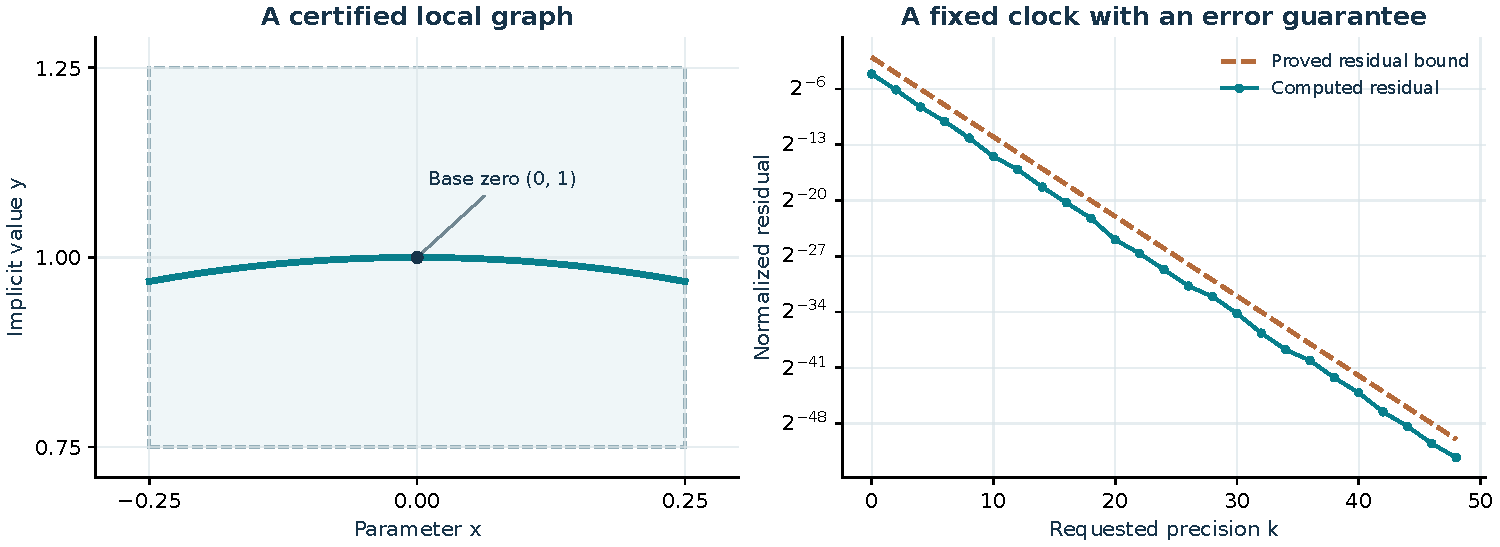
\includegraphics[width=\textwidth]{figures/implicit_graph.pdf}
 \caption{The circle example. Left: the certified rational box
 and the unique upper branch on the parameter interval.
 Right: exact-rational residuals from the implemented finite
 program, displayed on a logarithmic scale, together with the
 proved bound \(2^{-(k+2)}\). Floating-point conversion is used
 only to draw this figure; the validation inequalities use
 exact fractions.}
 \label{fig:circle}
\end{figure}

\subsection{A coupled two-dimensional vertical system}

To exhibit a matrix-valued vertical derivative, set
\[
 H(x,y_1,y_2)=
 \begin{pmatrix}
  y_1+\tfrac14y_1y_2-x\\
  y_2+\tfrac14y_1^2-\tfrac12x
 \end{pmatrix},
 \quad |x|\le\tfrac1{16},\quad |y_1|,|y_2|\le\tfrac14.
\]
The center is zero, \(A=\Id\), \(r=1/4\), \(M=1\), and
\[
 U=\begin{pmatrix}-1\\-1/2\end{pmatrix},\qquad
 V=\begin{pmatrix}
  1+y_2/4&y_1/4\\
  y_1/2&1
 \end{pmatrix}.
\]
Each row of \(\Id-V\) has absolute row sum at most \(1/8\).
The parameter condition is \(M\alpha=1/16=r/4\).
The Taylor remainders are \(k_1k_2/4\) and \(k_1^2/4\),
so their maximum is at most \(d^2/4\).
The full Jacobian changes by at most \(d/2\).
One may therefore take \(\mu_0(p)=\nu_0(p)=p\).
All raw certificates are rational polynomial inequalities.

The theorem gives a unique vector branch
\((g_1(x),g_2(x))\), Lipschitz constant \(2\), and the
explicit derivative equation
\[
 \begin{pmatrix}
  1+g_2/4&g_1/4\\
  g_1/2&1
 \end{pmatrix}
 \begin{pmatrix}g_1'\\g_2'\end{pmatrix}
 =\begin{pmatrix}1\\1/2\end{pmatrix}.
\]
The generic moduli are \(\mu_g(p)=p+5\) and
\(\nu_g(p)=p+6\).
The rational Neumann program computes this derivative
without needing a symbolic inverse formula.

\subsection{A simple nonlinear inverse with all assumptions discharged}

For an additional compact arithmetic instance, take
\[
 H(x,y)=y+y^3-x,\qquad
 |x|\le\tfrac1{16},\quad |y|\le\tfrac14.
\]
Here \(U=-1\), \(V=1+3y^2\), \(M=1\), and
\(|1-V|\le3/16\). The Taylor identity is
\[
 H(x+h,y+k)-H(x,y)+h-(1+3y^2)k=3yk^2+k^3.
\]
Because both vertical endpoints lie in the box,
\(|k|\le1/2\), and the remainder is at most
\((3/4+1/2)d^2\le2d^2\).
The derivative change is bounded by
\(3|y-y'||y+y'|\le(3/2)d\le2d\).
Thus \(\mu_0(p)=\nu_0(p)=p+1\) suffices.
The theorem constructs the unique local solution of
\[
 g(x)+g(x)^3=x,\qquad
 g'(x)=\frac1{1+3g(x)^2}.
\]
This instance needs only rational polynomial identities
and elementary order bounds; no pre-existing theorem
about cubic roots, implicit functions, or real completeness
is needed to discharge its input contracts.

\subsection{What the code verifies}

The executable implementation uses Python integers and
\code{fractions.Fraction}; it requires no third-party
packages. It implements \eqref{eq:algorithm} exactly and
uses explicitly bounded loops. The validation file contains
the deterministic results and hashes of the source files.

The supplied validation completed \(4{,}680\) traces:
two polynomial providers, nine parameter points per
provider, every requested precision from \(0\) through
\(64\), and four oracle modes. The additional modes add
controlled positive, negative, or varying errors of
size at most the allowed evaluation error.
The checks include \(168{,}480\) individual steps and
\(2{,}048\) aligned trace comparisons.

In total, \(1{,}317{,}978\) exact-rational assertions passed.
They check domain preservation, evaluation and rounding
budgets, the scaled recurrence invariant, the terminal
residual bound, parameter sensitivity, finite Neumann
identities, and derivative calculations against an
independent rational matrix inverse. Special cases exercise
negative dyadic flooring and clipping at both endpoints
of a non-dyadic interval. The circle example also has
independent exact polynomial root brackets.

These computations establish that the implementation and
the displayed constants agree on the tested cases.
They do not establish the universally quantified raw
certificates by sampling, and they are not an iPRA proof
checker. The mathematical proofs of the certificates
and general theorem are the algebraic arguments above;
the separate Lean core checks specific finite lemmas.

\section{Lean formalization and ProveIt integration}\label{sec:lean}

\subsection{Verification status}

The archive deliberately separates three kinds of evidence.
The manuscript contains the complete human-readable proof
and its iPRA induction audit. The executable code checks
the concrete finite algorithm on specified instances.
The file \code{lean/FiniteCore.lean} contains compiled
host-Lean proofs of finite arithmetic and algebra.
The complete implicit function theorem has not been
formalized in that file, and the archive does not contain
a completed \(\Prf\,\PRAAx\) derivation of the full theorem.

The Lean target imports only the bundled \code{Std}
library and was checked with Lean 4.32.0, compiler commit
\code{8c9756b28d64dab099da31a4c09229a9e6a2ef35}.
Both direct compilation and \code{lake build} succeeded.
The included compiler log records the kernel dependencies.
There are no \code{sorry} placeholders or user-declared
axioms in this checked target. Its reported dependencies
include \code{propext} and \code{Quot.sound}, and do not
include \code{Classical.choice}. This is a report about
the host proof terms; it is not a substitute for checking
the object theory in which a derivation is constructed.

The main checked declarations, in namespace
\code{ConstructiveIFT}, are:
\begin{center}
\small
\begin{tabular}{>{\raggedright\arraybackslash}p{0.42\textwidth}>{\raggedright\arraybackslash}p{0.50\textwidth}}
\toprule
Declaration & Content\\
\midrule
\code{errorBudget\_closed} &
Exact finite weighted geometric error sum.\\
\code{half\_contraction\_closed} &
The denominator-cleared inexact contraction inequality.\\
\code{half\_contraction\_budget\_finite} &
The bound using only the finite prefix of recurrence hypotheses.\\
\code{checked\_half\_contraction\_budget} &
A primitive-recursive-style Boolean trace checker implies
the finite bound.\\
\code{iterate\_add} &
Concatenation of two finite iteration segments.\\
\code{neumann\_residual} &
The finite vector identity \(z_N+E^Nb=Ez_N+b\), with
the required additive laws supplied explicitly.\\
\bottomrule
\end{tabular}
\end{center}

For example, the checked finite checker theorem has the form
\begin{lstlisting}
theorem checked_half_contraction_budget
    (d : Nat -> Nat) (e N : Nat)
    (checked : checkSteps d e N = true) :
    2 ^ N * d N <= errorBudget (d 0) e N
\end{lstlisting}
The host parameter \(d\) becomes a fixed primitive recursive
symbol in the object-language version. The checked theorem
does not by itself assert primitive recursiveness of an
arbitrary host function.

\subsection{The repository snapshot actually inspected}

The GitHub connector resolved ProveIt main to commit
\[
 \code{d36b35eed5bd01af4ade66bf539622495813ccc8}.
\]
The inspected sources and project status are recorded in
the archive's source manifest and audit. No repository
files were modified. The reference snapshot contains the
selected source modules, not their complete transitive
import closure, and those repository modules were not
rebuilt as part of this package.

The following paths are relative to
\path{Logic/PrimitiveRecursiveArithmetic/Derivations/Lean/IPRADerivations/}.
The source uses \(\Prf\,\PRAAx\), making it relevant to
object iPRA, rather than merely to analysis in host Lean.
\begin{center}
\small
\begin{tabular}{>{\raggedright\arraybackslash}p{0.35\textwidth}>{\raggedright\arraybackslash}p{0.57\textwidth}}
\toprule
Module & Inspected interface and reuse boundary\\
\midrule
\path{Foundations/ContractionTrace.lean} &
\code{contraction\_iter} uses an internal object index and
explicit \code{PRA.qfInd}. It is the best template for
the new additive-error trace invariant.\\[3pt]
\path{Analysis/HalfContractionTail.lean} &
Internal-index geometric and tail bounds, using a
nonincreasing finite potential.\\[3pt]
\path{Analysis/DyadicCauchy.lean} &
Closed object formulas for fixed primitive recursive
symbols with a particular adjacent dyadic-integer
motion hypothesis. An adapter to that format would
need proof; it is not automatic for our name.\\[3pt]
\path{Analysis/FiniteFTC.lean} &
Internal finite-mesh summation of signed local errors;
a suitable template for our polygon argument.\\[3pt]
\path{Foundations/ContractionIterates.lean} &
Internal exact-contraction iteration and Cauchy
templates. The rounded evaluator needs the inexact
adaptation.\\[3pt]
\path{Analysis/FeedbackInexact.lean} &
Genuine object proof terms, but the iteration count is
an external Lean index in the inspected theorem
family. It is not already the internally quantified
runtime loop theorem needed here.\\[3pt]
\path{Foundations/NeumannCorrection.lean} &
Genuine finite matrix identities in the object
theory, with an external truncation index.
An internal coded matrix loop is still required.\\
\bottomrule
\end{tabular}
\end{center}

These distinctions matter: an externally recursive family
of proof terms containing the numeral \(2^k\) is not the
same object theorem as a universally quantified bound
for variable \(k\). The existing modules supply valuable
proof patterns and elementary arithmetic, while the
new evaluator and the variable-length inexact argument
still require an integration layer.

\subsection{Required definitions in a full Lean development}

The detailed \code{lean/BLUEPRINT.md} accompanies this
section. A clean implementation has two connected levels.
Host Lean can use
\[
 \code{QVec n := Fin n -> Rat},\qquad
 \code{QMat m n := Fin m -> Fin n -> Rat},
\]
with explicit finite folds for norms. Object iPRA uses
their numerical list encodings. At either level the
necessary definitions are:
\begin{enumerate}
 \item Signed rational codes, their validity predicates,
 arithmetic, comparison, positive-denominator witnesses,
 and numerical definitions of finite vectors and matrices.
 \item Supremum and row-sum norms, product and triangle
 inequalities, boxes, dyadic floor, and clipping.
 \item Regular names, finite-observation equality and
 order, and the bounded-precision operations on names.
 \item The fixed evaluator symbols, raw certificates
 R0--R4, and the named-point extension programs with
 moduli \eqref{eq:rawenlarge}.
 \item The numerical trace function
 \eqref{eq:algorithm}, its clock \(N(k)\), and the finite
 prefix checker for local error inequalities.
 \item The primitive recursive graph evaluator,
 parameter-name composition, residual observation
 formulas, and quantitative uniqueness formulas.
 \item Coded matrix powers, finite Neumann sums, their
 rational perturbation bounds, and the derivative
 evaluator \eqref{eq:derivativeprogram}.
 \item The numerical Taylor and continuity output
 formulas with \(\mu_g,\nu_g\), and the rational
 preconditioner construction.
\end{enumerate}
All these definitions have been specified mathematically
above. None requires an unspecified function-space
quantifier in the arithmetic language.

\subsection{A concrete completion order}

\paragraph{1. Rational arithmetic and finite arrays.}
Implement the encodings and prove their primitive
recursive definitions satisfy the elementary field
identities under the denominator guards. Keep the
algorithmic rational operations shared between the
producer and the certificate checker. Prove clipping
nonexpansive by rational order cases.

\paragraph{2. The internally quantified inexact trace theorem.}
Port the integer invariant from the checked core to
\(\Prf\,\PRAAx\), using the internal-index method in
\code{ContractionTrace}. The induction formula is the
Boolean-prefix-check implication to the integer
invariant. This is the first main proof obligation
not already discharged by the supplied host-Lean file.

\paragraph{3. The raw Taylor-to-segment adapter.}
Implement \(L_p\), the finite rational polygon, and
the error budget at a fixed observation precision.
Use the finite signed-sum pattern in \code{FiniteFTC}.
Prove rational squeezing and instantiate it to obtain
the one-step contraction estimates for actual program
outputs. This step connects analytic input certificates
to the finite trace theorem.

\paragraph{4. The implicit-function name.}
Define the rounded trace by primitive recursion.
Use aligned final segments and the inexact trace
theorem to prove \eqref{eq:pairbound}; use adjacent
increments to prove \eqref{eq:residual}.
Build the regular output name directly. Then prove
the zero equation, uniqueness, residual bound,
Lipschitz estimate, and the parameter-name extension.
No separate theorem about an arbitrary complete
metric space is needed.

\paragraph{5. Internally variable finite matrix loops.}
Encode a matrix as a fixed-length numerical array.
Use componentwise rational loop invariants to prove
the two geometric identities and the power-difference
identity. The source in \code{NeumannCorrection}
provides exact finite algebra, but its external index
must be replaced by the coded internal loop. Prove
the finite norm sums \(2,4,8\) needed in
Lemma~\ref{lem:perturb}.

\paragraph{6. The \(C^1\) conclusion.}
Compose the Jacobian evaluator with the graph name at
the explicit index \(\nu(q+1)\), construct the
derivative name from a Neumann sum, and translate the
Taylor calculation and inverse-difference calculation
at arbitrary fixed output precision. This supplies
the exact formulas \(\mu_g,\nu_g\). Finally formalize
the determinant-apartness and translated-center
adapters.

\paragraph{7. Object-proof audit and an optional classical bridge.}
The final target should be an actual
\(\Prf\,\PRAAx\) object derivation of the finite
observation schema, with each induction constructor
carrying a verified quantifier-free formula.
Audit its dependency closure for placeholders and
unintended assumptions. A subsequent interpretation
in ordinary real analysis may use Mathlib's real
vectors and calculus to compare with its existing
implicit function theorems \cite{mathlib}.
Such a comparison is useful, but invoking Mathlib's
noncomputable implicit-function construction would
not establish the primitive recursive output or
the restricted-induction claim.

\subsection{Reproduction}

From the package root, run
\begin{lstlisting}
python3 code/validate.py
cd lean
lake build
\end{lstlisting}
The project pins Lean 4.32.0. To rebuild the report,
from the \code{paper} directory run
\begin{lstlisting}
pdflatex -interaction=nonstopmode -halt-on-error implicit_function_ipra.tex
pdflatex -interaction=nonstopmode -halt-on-error implicit_function_ipra.tex
\end{lstlisting}
The figure is already included. Its optional regeneration
script uses Matplotlib; Matplotlib is not required by
the rational solver or its validation suite.

\section{Provenance and references}

The target classical theorem was the finite-dimensional
\(C^1\) implicit function theorem described in the user's
linked overview \cite{wikipedia}. The proof here was
developed directly from quantitative rational certificates.
The constructive literature \cite{diener2011,diener2009}
provides context for the role of quantitative uniqueness.
The classical article \cite{oliveira} is a useful
comparison, not a foundational premise of this proof.

The ProveIt sources were inspected at the exact commit
specified in Section~\ref{sec:lean}. Their relevant
interfaces and limitations are documented in
\code{references/proveit/repo\_audit.md}; the accompanying
manifest gives a commit-pinned URL and blob hash for
each copied reference source. These files are evidence
for the reuse assessment and are not part of the
self-contained \code{FiniteCore} build target.

\begingroup
\raggedright
\begin{thebibliography}{9}

\bibitem{diener2011}
H. Diener and P. Schuster,
\emph{Uniqueness, continuity and the existence of implicit
functions in constructive analysis},
LMS Journal of Computation and Mathematics \textbf{14}
(2011), 127--136.
\url{https://doi.org/10.1112/S1461157010000057}.

\bibitem{diener2009}
H. Diener and P. Schuster,
\emph{Uniqueness, Continuity, and Existence of Implicit
Functions in Constructive Analysis},
in CCA 2009, OASIcs \textbf{11}, 131--140.
\url{https://doi.org/10.4230/OASIcs.CCA.2009.2265}.

\bibitem{oliveira}
O. Rio Branco de Oliveira,
\emph{The Implicit and the Inverse Function theorems:
easy proofs},
Real Analysis Exchange \textbf{39}(1) (2013/2014),
207--218; arXiv:1212.2066.
\url{https://arxiv.org/abs/1212.2066}.

\bibitem{proveit}
V. Reshetnikov and contributors,
\emph{ProveIt: Logic/PrimitiveRecursiveArithmetic},
snapshot at commit
\code{d36b35eed5bd01af4ade66bf539622495813ccc8}.
\url{https://github.com/VladimirReshetnikov/ProveIt/tree/d36b35eed5bd01af4ade66bf539622495813ccc8/Logic/PrimitiveRecursiveArithmetic}.
Selected object-theory derivation sources are listed
in the package manifest.

\bibitem{mathlib}
The Mathlib community,
\emph{Mathlib.Analysis.Calculus.ImplicitContDiff},
official documentation, inspected November 21, 2026.
\url{https://leanprover-community.github.io/mathlib4_docs/Mathlib/Analysis/Calculus/ImplicitContDiff.html}.
The documentation identifies
\code{ContDiffAt.implicitFunction} as noncomputable
and gives its smoothness and local inverse properties.

\bibitem{wikipedia}
\emph{Implicit function theorem},
Wikipedia, user-specified overview, inspected
November 21, 2026.
\url{https://en.wikipedia.org/wiki/Implicit_function_theorem}.

\end{thebibliography}
\endgroup

\end{document}
